\chapter{Results}
\label{ch:results}

In the results chapter, you present your findings and experimental results: Briefly reintroduce the research questions or hypotheses and explain the structure of the results section. State how the data were analyzed without going into the depth of the methodology.

It is important to focus on the presentation: Include tables, figures, or graphs --- but describe the results as well in the text and help the reader understand what is shown in the figure and what is noteworthy (see example Fig. \ref{} and the text description is moved to the caption). It is often necessary to select which figures to show. It is usually best to start with a general overview of the results for that experiments (e.g., showing a learning curve), before highlighting a specific finding and presenting more detailed data supporting this result. 

In the following, I just give briefly examples for results (all taken from ):
\begin{itemize}
\item A result figure, showing a learning curve: Fig. \ref{fig_res_learning_curves};
\item An example for a table comparing evaluation results for different learning architectures in table \ref{tab_res_characteristics};
\end{itemize}



\begin{figure}[tb]
\centering
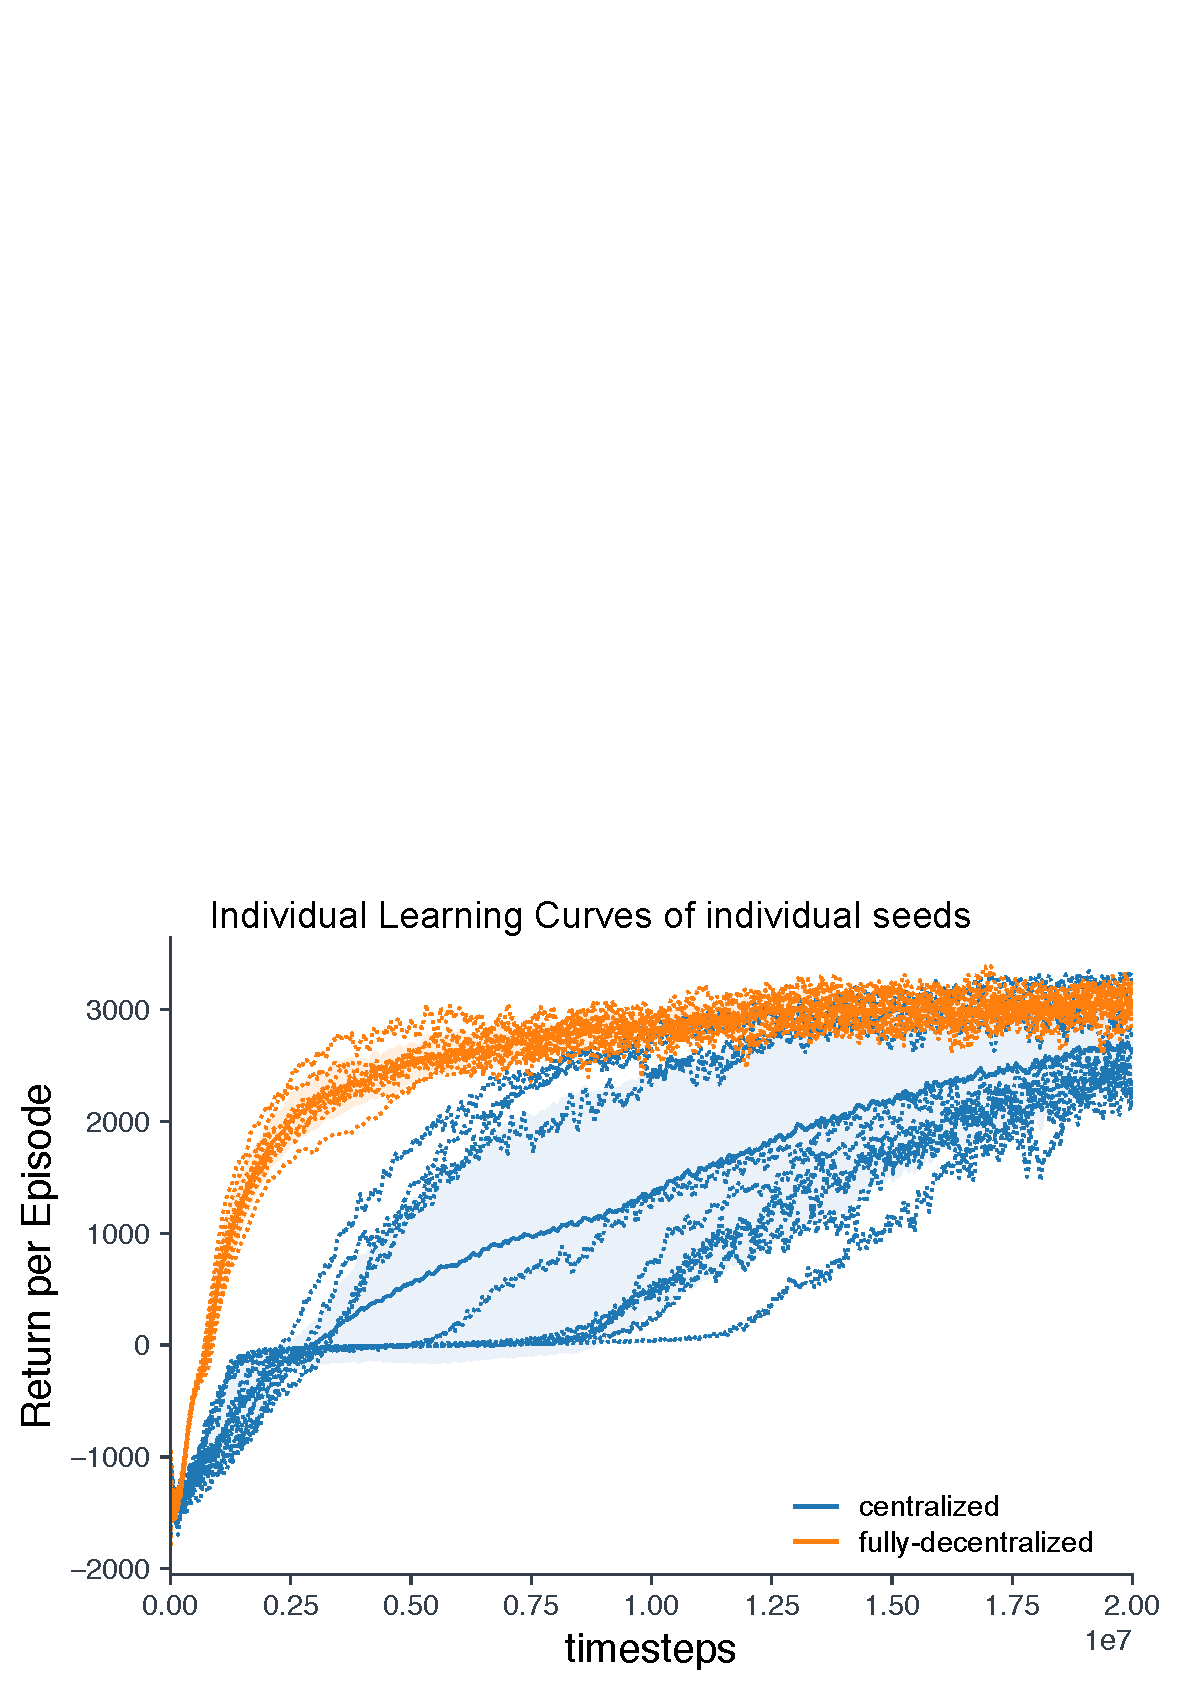
\includegraphics[width=0.7\columnwidth]{img/07_LearningCurves.pdf}%
\caption{Learning curves for different controller architectures over learning time: Individual learning curves for centralized (blue) and fully decentralized (orange) controller architecture over learning time, given in simulation steps on the x-axis (interactions with the environment) and shown is the return per episode on the y-axis. Explanation in text: While all approaches were able to learn walking behavior, learning progressed quite differently for the different architectures (see learning curves in Fig. \ref{fig_res_learning_curves}). The centralized approach shows worse learning characteristics. First, return is increasing much slower compared to the decentralized architectures. Second, variance becomes very large for a considerable time of training.}
\label{fig_res_learning_curves}
\end{figure}

\begin{table*}[tbh]
\centering
\ra{1.1}
\captionsetup{format =hang}%

\caption{Evaluation of different control architectures. Each architecture was trained $10$ times and each of these seeds was evaluated for $100$ episodes on multiple different terrains (flat terrain; uneven terrain, smoothness $0.8$; bumpy terrain, smoothness $0.6$). Given is the mean return, mean velocity, and cost of transport over all episodes per architecture for a specific terrain type. Shown are the different control architectures.}

\begin{adjustbox}{center}
\begin{tabular}{lcccccccccccc@{}}
%\begin{tabular}{lccc}
\toprule
Configuration & & \multicolumn{3}{c}{Flat terrain} &\phantom{a} & \multicolumn{3}{c}{Uneven terrain (0.8)} &\phantom{a} & \multicolumn{3}{c}{Bumpy terrain (0.6)} \\  
\cmidrule{3-5} \cmidrule{7-9}  \cmidrule{11-13} 
&& Return & Vel. & CoT && Return & Vel. & CoT && Return & Vel. & CoT  \\
\midrule
 \parbox[l]{2.4cm}{Fully Decentr. \\ (4 controller)} &
\parbox[c]{0.8cm}{\vspace{0.05cm}
\includegraphics[width=0.8cm]{img/Controller_Config_1.pdf}\vspace{0.05cm}} & 2673.0 & 3.33 & 6.283 && 974.0 & 2.15 & 7.424 && -137.5 & 0.64 & 14.099\\
\hline
\parbox[l]{2.4cm}{Decentr. local\\ inf., both n.} &
\parbox[c]{0.8cm}{\vspace{0.05cm}
\includegraphics[width=0.8cm]{img/Controller_Config_3.pdf}\vspace{0.05cm}} & 2943.4 & 3.54 & 6.169 && 1447.0 & 2.55 & 7.283 && 276.4 & 1.20 & 11.357 \\
 \hline
\parbox[l]{2.4cm}{Centralized \\ single contr.}&
\parbox[c]{0.8cm}{\vspace{0.05cm}
\includegraphics[width=0.8cm]{img/Controller_Config_4.pdf}\vspace{0.05cm}} & 2605.9 & 3.57 & 8.224 && 1110.5 & 2.55 & 9.324 && 201.5 & 1.36 & 12.641\\

\bottomrule
\end{tabular}
\end{adjustbox}
\label{tab_res_characteristics}
\end{table*}

\clearpage

\section{Tips for Presenting Results Effectively}
\begin{itemize}
    \item \textbf{Stay Objective:} Report what the data shows without adding personal interpretation or bias. Leave analysis for the discussion section.
    \item \textbf{Use Visuals Wisely:} Employ graphs, charts, and tables to illustrate your results clearly. Make sure each visual is relevant, properly labeled, and mentioned in the text.
    \item \textbf{Be Clear and Concise:} Avoid cluttering the section with unnecessary details. Focus on presenting the results that directly pertain to your research questions.
    \item \textbf{Consistent Formatting:} Use a consistent format for presenting data. This includes similar styles and scales for graphs, consistent decimal places for numbers, and uniform units of measure.
    \item \textbf{Highlight Significant Results:} Clearly point out the most important findings of your research. Emphasize results that are statistically significant or particularly relevant to your research questions.
    \item \textbf{Explain Variability:} If there are anomalies or a high degree of variability in your data, provide a brief explanation or note that this will be discussed further in the discussion section.
\end{itemize}

